\newpage

\section{Mourning Tweets}

El desarrollo y código fuente de esta sección de la tarea se encuentra en el cuaderno \texttt{HW02\_4.ipynb} adjunto.

\subsection{Mourning Lexicon}

\subsubsection{Procesamiento de los \textit{Tweets}}

Antes de realizar la construcción de los \textit{Lexicones} e implementar los modelos de clasificación se realizó un proceso estándar para \textit{tokenizar} los \textit{tweets}. Para esto se hizo un procesamiento especial pensado en lenguaje especifico que se utiliza en \textit{Twitter} y las particularidades de ruido que este medio conlleva. Para esto se realizaron los siguientes pasos:

\begin{itemize}
    \item Remover la puntuación de los \textit{Tweets}.
    
    \item \textit{Tokenizar} el \textit{dataset} con el \textit{tokenizador} (\texttt{TweetTokenizer}) de \texttt{nltk} especializado para este tipo de datos. Esta herramienta:
    \begin{itemize}
        \item Estandariza todas las palabras a minúsculas.
        
        \item Reduce la longitud de las palabras en caso de repetir letras.
        
        \item Remueven caracteres especiales de \textit{Twitter} y usuarios (\textit{@}).
    \end{itemize}
    
    \item Remover las \textit{stop\_words} utilizando el set de palabras de \texttt{nltk} para cada uno de los idiomas (inglés y español).
    
    \item Con los términos (\textit{tokens}) de los \textit{tweets} se construye un vocabulario (o \textit{dictionary}) para cada uno de los \textit{datasets} (inglés y español). 
    
    \item Filtrar términos poco comunes (aquellos que aparecen en menos de 5 \textit{tweets}) y muy comunes (aquellos que aparecen en más del 75\% del \textit{dataset}). Para esto se uso la función \texttt{filter\_extremes} de \texttt{Gensim}. Esto resulto en vocabularios de alrededor de 5000 palabras para ambos idiomas.
    
\end{itemize}

\subsubsection{Construcción de lexicones}

Una vez se tienen definido el diccionario para los dos datasets, se construyen los lexicones estimando la probabilidad de que cada uno de los términos (\textit{tokens}) este en cada clase (luto o no luto). En este caso, la clase \textbf{luto \textit{(mourning)} se modela como la clase positiva} ($c = 1$) y la clase de \textbf{no luto \textit{(no mourning)} se modela como la clase negativa} ($c = 0$). \\

Para estimar dichas probabilidades, se utilizan los conceptos de verosimilitud  (\textit{likelihood}) y de verosimilitud escalada (\textit{scaled likelihood}). Las expresiones para dichas probabilidades son adaptadas de la referencia \cite{Potts2010SALT}, y se presentan a continuación:

\begin{equation}
    \mathbf{P(w|c=i)} = \frac{f(w,c=i)}{\sum_{w\in C} f(w,c=i)}
    \label{likelihood}
\end{equation} 

Al escalar esta probabilidadc condicional con las probabilidades \textit{a priori} de las palabras y las clases (utilizando el teorema de Bayes), se obtiene la siguiente probabilidad condicional:

\begin{equation}
    \mathbf{P(c=i|w)} = \frac{P(w|c=i) p(c=i)}{p(w)} = \frac{P(w|c=i)}{\sum_{c\in C} P(w|c=i)}
    \label{scaled_likelihood}
\end{equation} 

En \cite{Potts2010SALT}, sugieren trabajar con esta segunda probabilidad condicional pues un sentido más acorde. Dada la palabra, cual es la probabilidad que pertenezca a la clase. No obstante, para los dataset en cuestión se analizan ambas probabilidades.

\subsubsection{Resultados}
A partir de las expresiones (\ref{likelihood}) y (\ref{scaled_likelihood}), se calculan las probabilidades de cada termino para la clase mourning ($c=1$) en los dos datasets (inglés y español).

\begin{table}[H]
    \centering
    \caption{Resultado de los 15 términos con mayor probabilidad de aparecer en tweets de luto (\textit{mourning}) del \textit{dataset} en español (ES).}
    \label{tab:es_lexicons}
    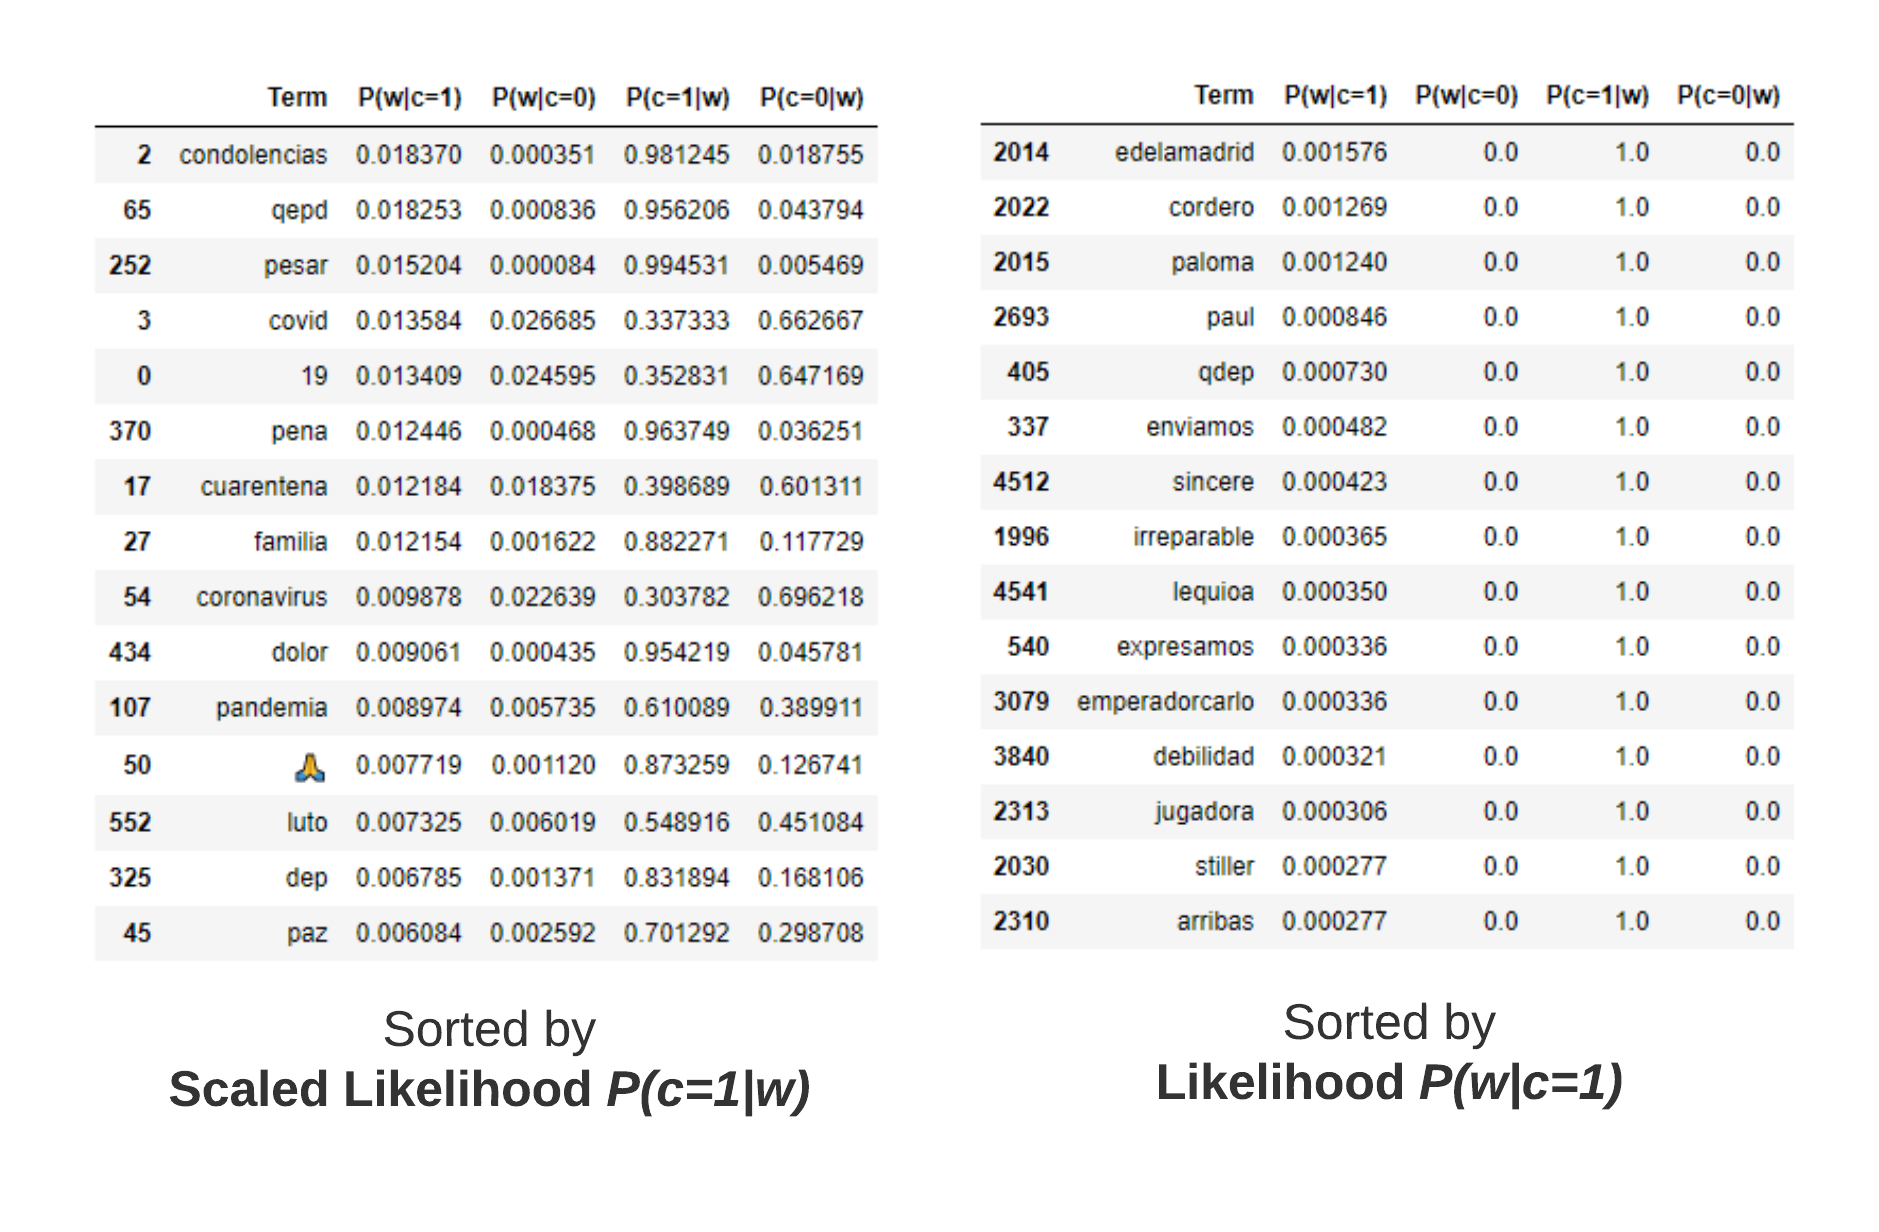
\includegraphics[width=\textwidth]{doc/images/ES_Lexicons.png}
\end{table}

\begin{table}[H]
    \centering
    \caption{Resultado de los 15 términos con mayor probabilidad de aparecer en tweets de luto (\textit{mourning}) del \textit{dataset} en inglés (EN).}
    \label{tab:en_lexicons}
    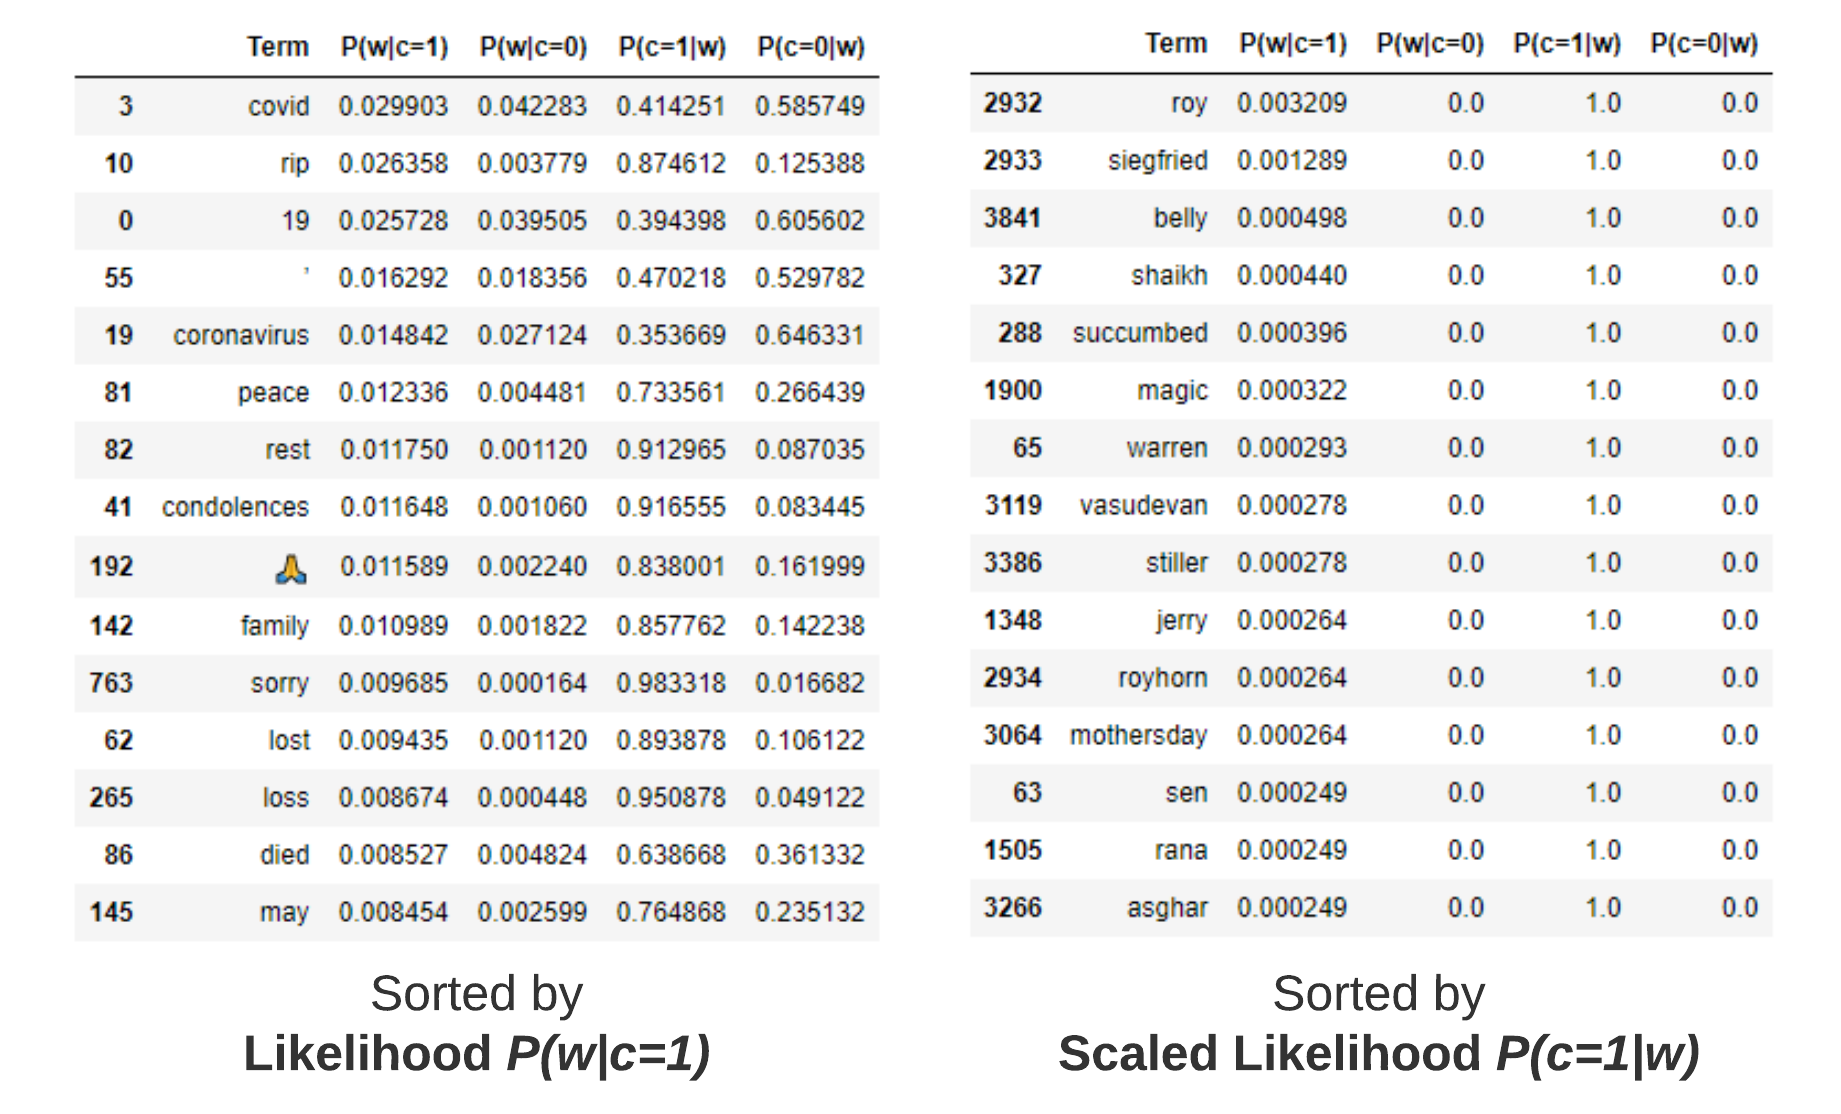
\includegraphics[width=\textwidth]{doc/images/EN_Lexicons.png}
\end{table}

En los cuadros \ref{tab:es_lexicons} y \ref{tab:en_lexicons} se observan los 15 términos con mayor probabilidad de pertenecer a un \textit{tweet} de luto para el \textit{dataset} en español y en inglés, respectivamente. En ambos casos se presentan los resultados ordenados tanto por su \textit{likelihood} (probabilidad $P(w|c=1)$) como por \textit{scaled likelihood} (probabilidad $P(c=1|w)$). En general los resultados son bastante similares en ambos idiomas, especialmente si se mira solo su probabilidad sin escalar. \\

En este caso, y a pesar de no estar ordenados exactamente igual, se observan términos muy similares en ambos idiomas. Acrónimos de luto como \textit{qdep}, el emoticón de las manos orando (id 50) y palabras como condolencias, pena, paz y familia (\textit{rip, condolences, peace, family, sorry}) se encuentran en ambas listas. De igual forma, al organizar los términos únicamente por esta probabilidad, se encuentran también palabras asociadas a la pandemia como coronavirus, covid, 19 en ambos idiomas. No obstante, es evidente que estos términos se encuentran ahí por su alta frecuencia a lo largo de todos los \textit{tweets}. Esto se puede afirmar poque, aunque su probabilidad condicional de pertenecer a la clase de luto $P(w|c=1)$ es muy alta, también lo es su probabilidad de pertenecer a la clase de no luto $P(w|c=0)$, e incluso en algunos casos es mayor. \\

Por otro lado, si se observan los términos ordenados por la probabilidad escalada $P(c=1|w)$ se obtiene una lista de palabras poco comunes. Esto se debe a que al escalar por la probabilidad de la palabra (dividir entre $p(w)$), las palabras poco comunes obtienen un peso muy importante. De hecho, el set de palabras que se obtiene, tiene en todos los términos la misma probabilidad (1). Esto quiere decir que son palabras que solo aparecen en la clase de luto (\textit{mourning}), a pesar de que su ocurrencia es realmente baja. 

\begin{table}[H]
    \centering
    \caption{Resultado de los 15 emoticones con mayor probabilidad de aparecer en tweets de luto (\textit{mourning}) del \textit{dataset} en español (ES).}
    \label{tab:es_emojis}
    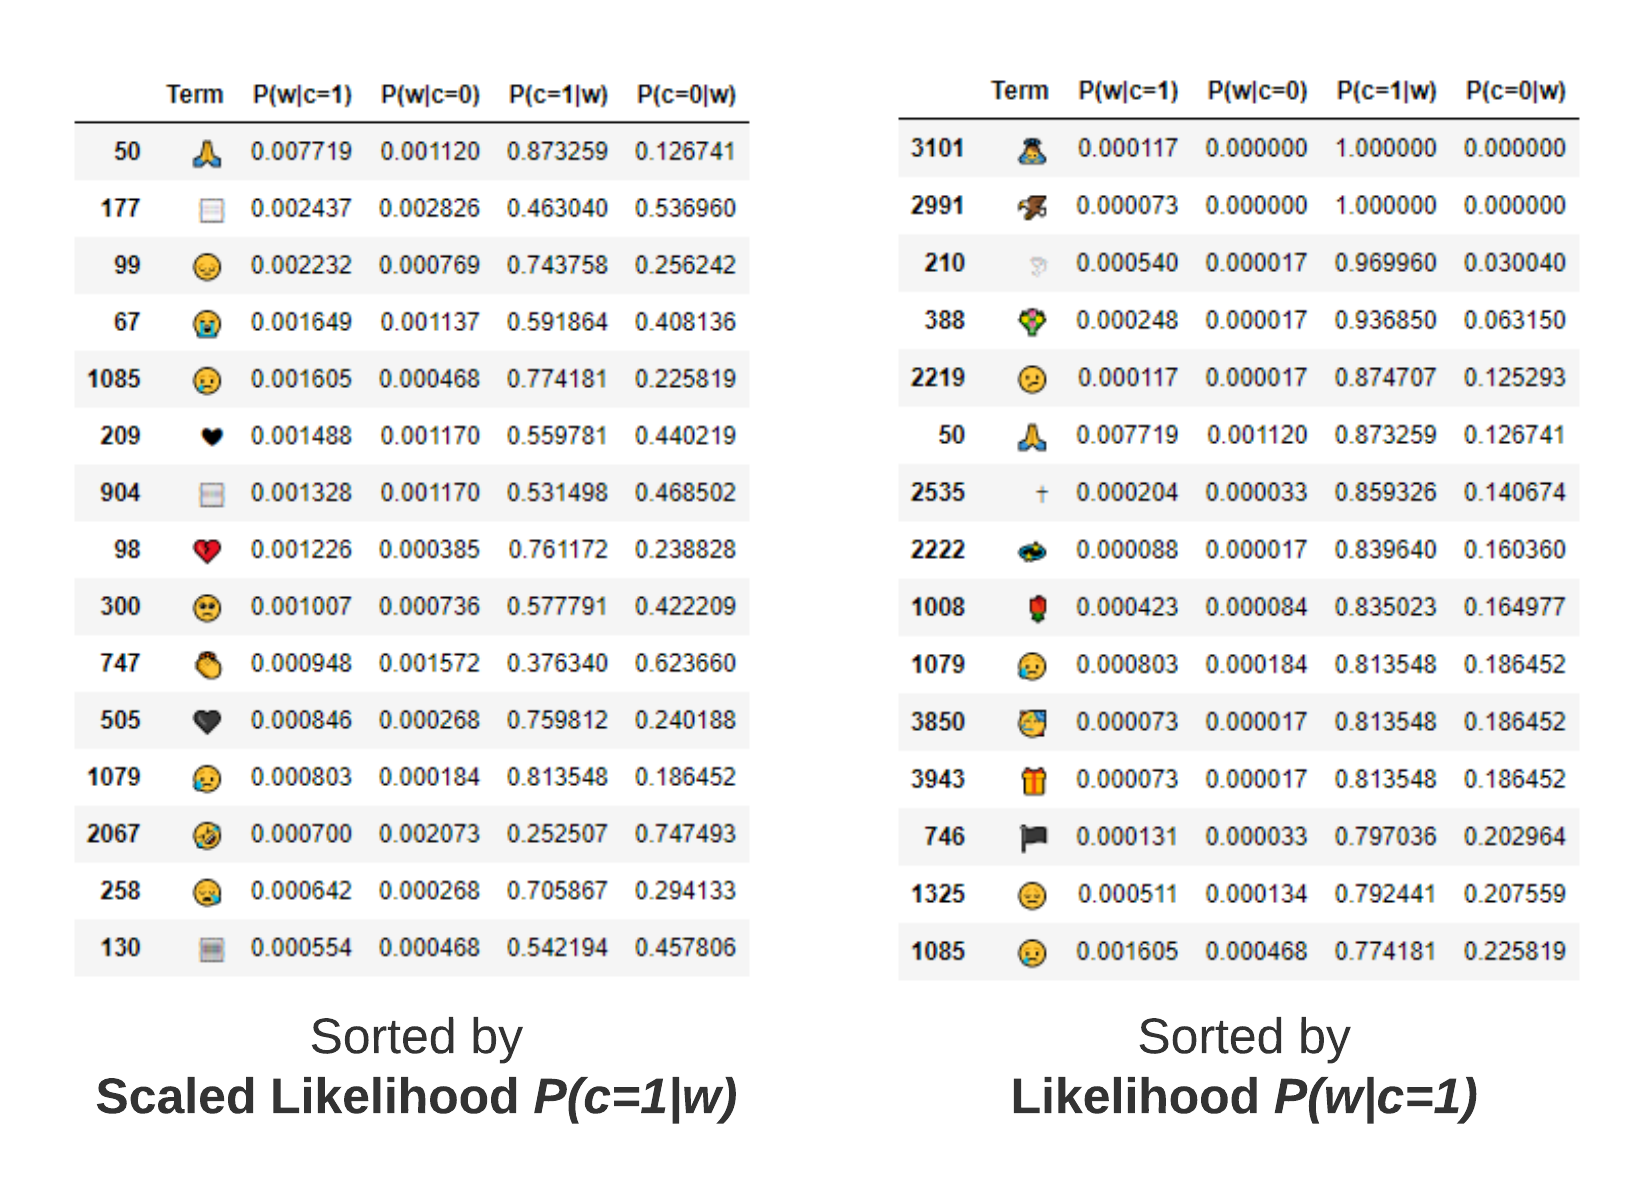
\includegraphics[width=\textwidth]{doc/images/ES_Emojis.png}
\end{table}

Ahora bien, algo similar a lo que ocurre con las palabras ocurre con los emoticones (véase cuadros \ref{tab:es_emojis} y \ref{tab:en_emojis}). Al mirar solo la lista ordenada por la probabilidad $P(w|c=1)$ se observan emoticones similares como: caritas tristes y llorando y corazones rotos y negros, en los \textit{datasets} de ambos idiomas. Adicionalmente, en ambos casos las manos orando encabezan la lista. No obstante, al ordenar por la probabilidad $P(c=1|w)$, se obtienen algunos emoticones poco comunes (como el guante de boxeo y el águila), cuya probabilidad es 1, pues solo aparecen en los \textit{tweets} de luto a pesar de su baja frecuencia. Sin embargo, empiezan a aparecer algunos otros con un sentido más relacionado al luto, como la paloma blanca, la cruz, un ángel y las flores. 

\begin{table}[H]
    \centering
    \caption{Resultado de los 15 emoticones con mayor probabilidad de aparecer en tweets de luto (\textit{mourning}) del \textit{dataset} en español (ES).}
    \label{tab:en_emojis}
    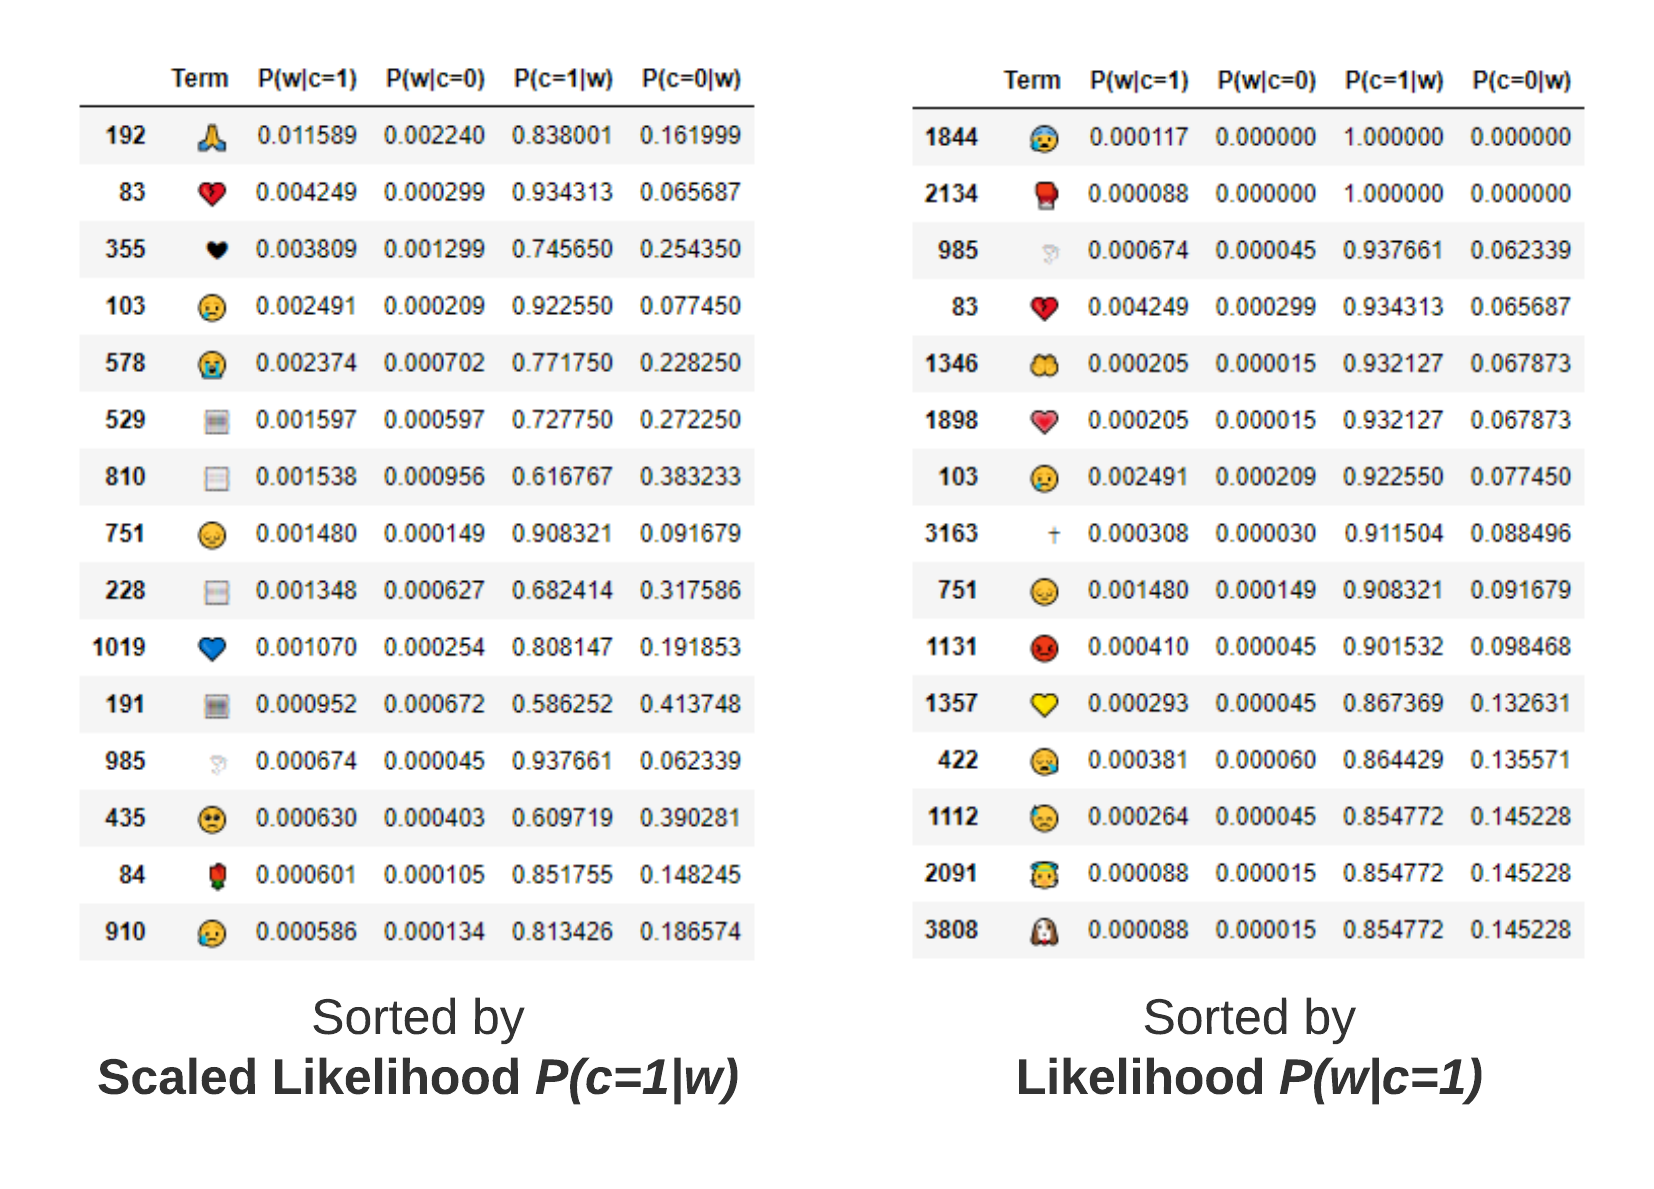
\includegraphics[width=\textwidth]{doc/images/EN_Emojis.png}
\end{table}

\subsection{Clasificadores}

\subsubsection{Representación de características}

Para poder entrenar un modelo de clasificación binario (clasificación de \textit{tweet} como luto o no luto) fue necesario convertir los \textit{tweets tokenizados} en un modelo de bolsa de palabras (\textit{BOW Model}). Esto permitirá después obtener información sobre los términos (\textit{tokens}) más relevantes para algunos de los modelos entrenados como clasificadores. \\

De igual forma, para poder evaluar el efecto de los emoticones (\textit{emojis}) en el entrenamiento, se construyeron dos representaciones de \textit{BOW}, una que los incluyera y otra que no. En total los emoticones (después del procesamiento de los \textit{tweets}) representaron aproximadamente un 3\% de los \textit{tokens} del vocabulario (alrededor de 150 términos en ambos idiomas). Por lo que el modelo BOW sin emoticones era de un tamaño ligeramente menor.

\subsection{Resultados}

Para entrenar los modelos se utilizó el 75\% de los datos y el resto del \textit{dataset} (25\%) se utilizó para poner a prueba el desempeño de los modelos presentado a continuación. En total se hicieron pruebas con 4 tipos de modelos (\textit{Naive Bayes, Logistic Regression, Decision Trees} y \textit{Random Forest}). Pero se entrenaron un total de 16 Modelos, dividendo las pruebas por idioma y por representación de caracteristicas (Modelos BOW que incluían o no los emoticones).

\begin{figure}[H]
    \centering
    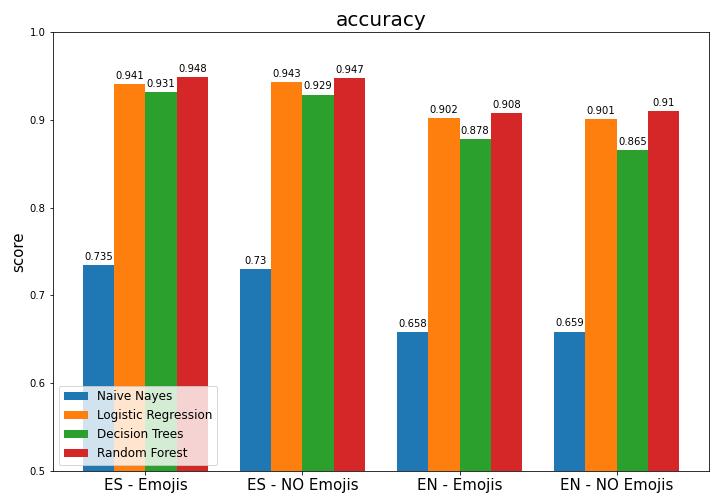
\includegraphics[width=0.8\textwidth]{results/mourning_tweets_accuracy.png}
    \caption{Resultados de \textit{Accuracy} para los distintos clasificadores sobre las distintas pruebas realizadas (\textit{datasets} en ingles y español y \textit{features} que incluyen o no \textit{emojis}.}
    \label{fig:mt_acc}
\end{figure}


\begin{figure}[H]
    \centering
    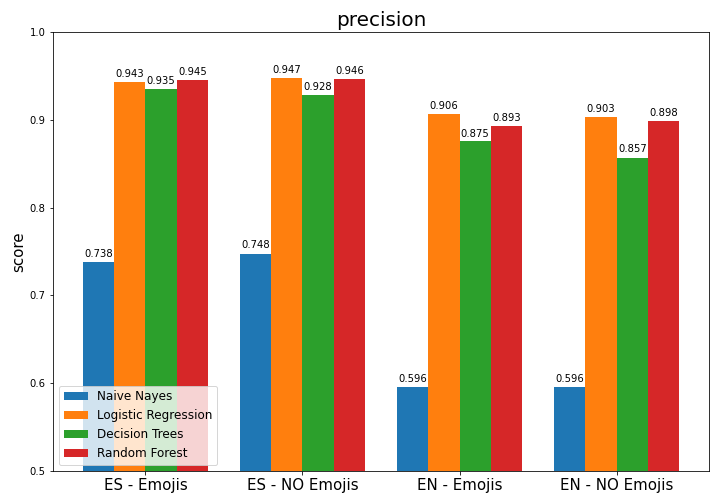
\includegraphics[width=0.8\textwidth]{results/mourning_tweets_precision.png}
    \caption{Resultados de \textit{Precision} para los distintos clasificadores sobre las distintas pruebas realizadas (\textit{datasets} en ingles y español y \textit{features} que incluyen o no \textit{emojis}.}
    \label{fig:mt_precision}
\end{figure}


\begin{figure}[H]
    \centering
    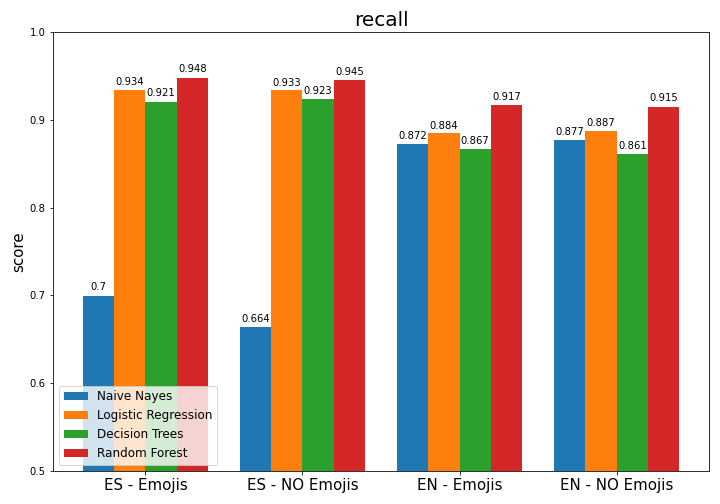
\includegraphics[width=0.8\textwidth]{results/mourning_tweets_recall.png}
    \caption{Resultados de \textit{Recall} para los distintos clasificadores sobre las distintas pruebas realizadas (\textit{datasets} en ingles y español y \textit{features} que incluyen o no \textit{emojis}.}
    \label{fig:mt_recall}
\end{figure}


\begin{figure}[H]
    \centering
    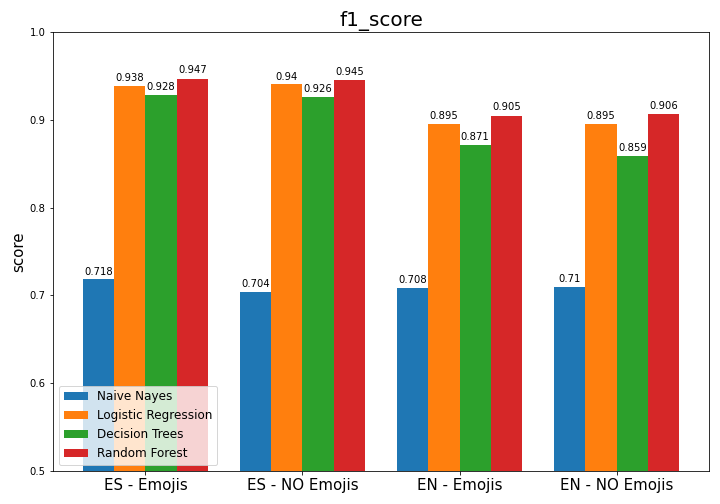
\includegraphics[width=0.8\textwidth]{results/mourning_tweets_f1_score.png}
    \caption{Resultados de \textit{F1 Score} para los distintos clasificadores sobre las distintas pruebas realizadas (\textit{datasets} en ingles y español y \textit{features} que incluyen o no \textit{emojis}.}
    \label{fig:mt_f1score}
\end{figure}

En términos generales se obtuvieron resultados bastante adecuados para una tarea de clasificación binaria. No obstante, que en todas las métricas el desempeño del clasificador de \textit{Naive Bayes} es considerablemente peor en todos los casos. Sin embargo, vale la pena destacar que su precisión aumenta bastante en el \textit{dataset} en español y su \textit{recall} aumenta considerablemente en el \textit{dataset} en inglés. \\

Por su parte los otros 3 clasificadores tienen desempeños bastante respetables, todos por encima del 90\% en casi todas las métricas. Siendo el \textit{Random Forest} el mejor clasificador, seguido del \textit{Logistic Regression} con un desempeño muy similar. Adicionalmente, también se puede observar que la tarea de clasificación fue ligeramente más difícil en inglés, pues en todos los casos se puede observar casi un 4\% de diferencia de desempeño en todas las métricas con el idioma español. En el cuadro \ref{tab:clf_summary} se puede observar un resumen de todos los resultados promedio obtenidos para cada uno de los clasificadores.


\begin{table}[H]
    \centering
    \caption{Resumen de resultados (métricas de desempeño) según clasificador y según idioma del \textit{dataset}}
    \label{tab:clf_summary}
    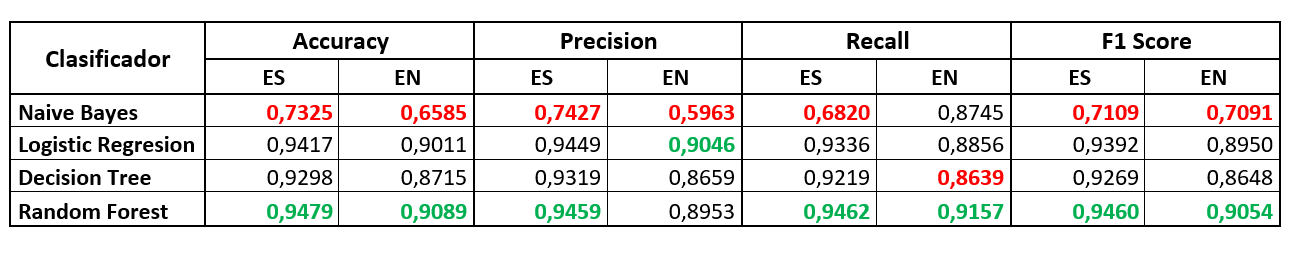
\includegraphics[width=\textwidth]{doc/images/summary_results_clf.png}
\end{table}

Ahora bien, en cuanto a la importancia de los emoticones, en el cuadro \ref{tab:emojis_summary} se puede observar el resultado promedio de todos los clasificadores agrupado por la inclusión o no de estos en su modelo de representación (\textit{BOW Model}). Aunque en casi todos los casos (salvo por la precisión en el idioma español) la inclusión de emoticones represento un mejor desempeño, en general la mejora es marginal y está lejos de ser categórica. Esto se puede deber al tamaño del \textit{dataset}, el cual es relativamente pequeño, pues aunque los emoticones brinden mayor información al problema, también pueden agregar un poco de ruido a la clasificación. No obstante, en términos generales se puede observar que su inclusión mejora el desempeño en ambos idiomas. 

\begin{table}[H]
    \centering
    \caption{Resumen de resultados (métricas de desempeño) según el \textit{set} de características (emojis o no emojis) utilizado para la clasificación y según el idioma.}
    \label{tab:emojis_summary}
    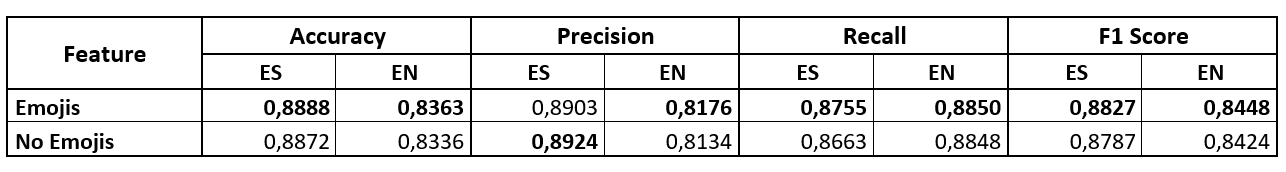
\includegraphics[width=\textwidth]{doc/images/summary_results_emoji.png}
\end{table}

\subsection{Análisis de importancia de características}

Finalmente, se desea evaluar que términos o emoticones son relevantes para la clasificación a partir de los modelos construidos. Esto con el fin de comparar estos resultados con los de los lexicones construidos anteriormente (véase literal 4.2). Para esto se evaluaron los parámetros de la regresión logística (LR) y del modelo de \textit{Random Forest} (RF). Los cuales se presentan a continuación

\subsubsection{Logistic Regression (LR)}

\begin{table}[H]
    \centering
    \caption{Términos con mayor peso dentro de los parámetros de Regresión Logística (LR) en el \textit{dataset} en español (ES)}
    \label{tab:lr_coef_es}
    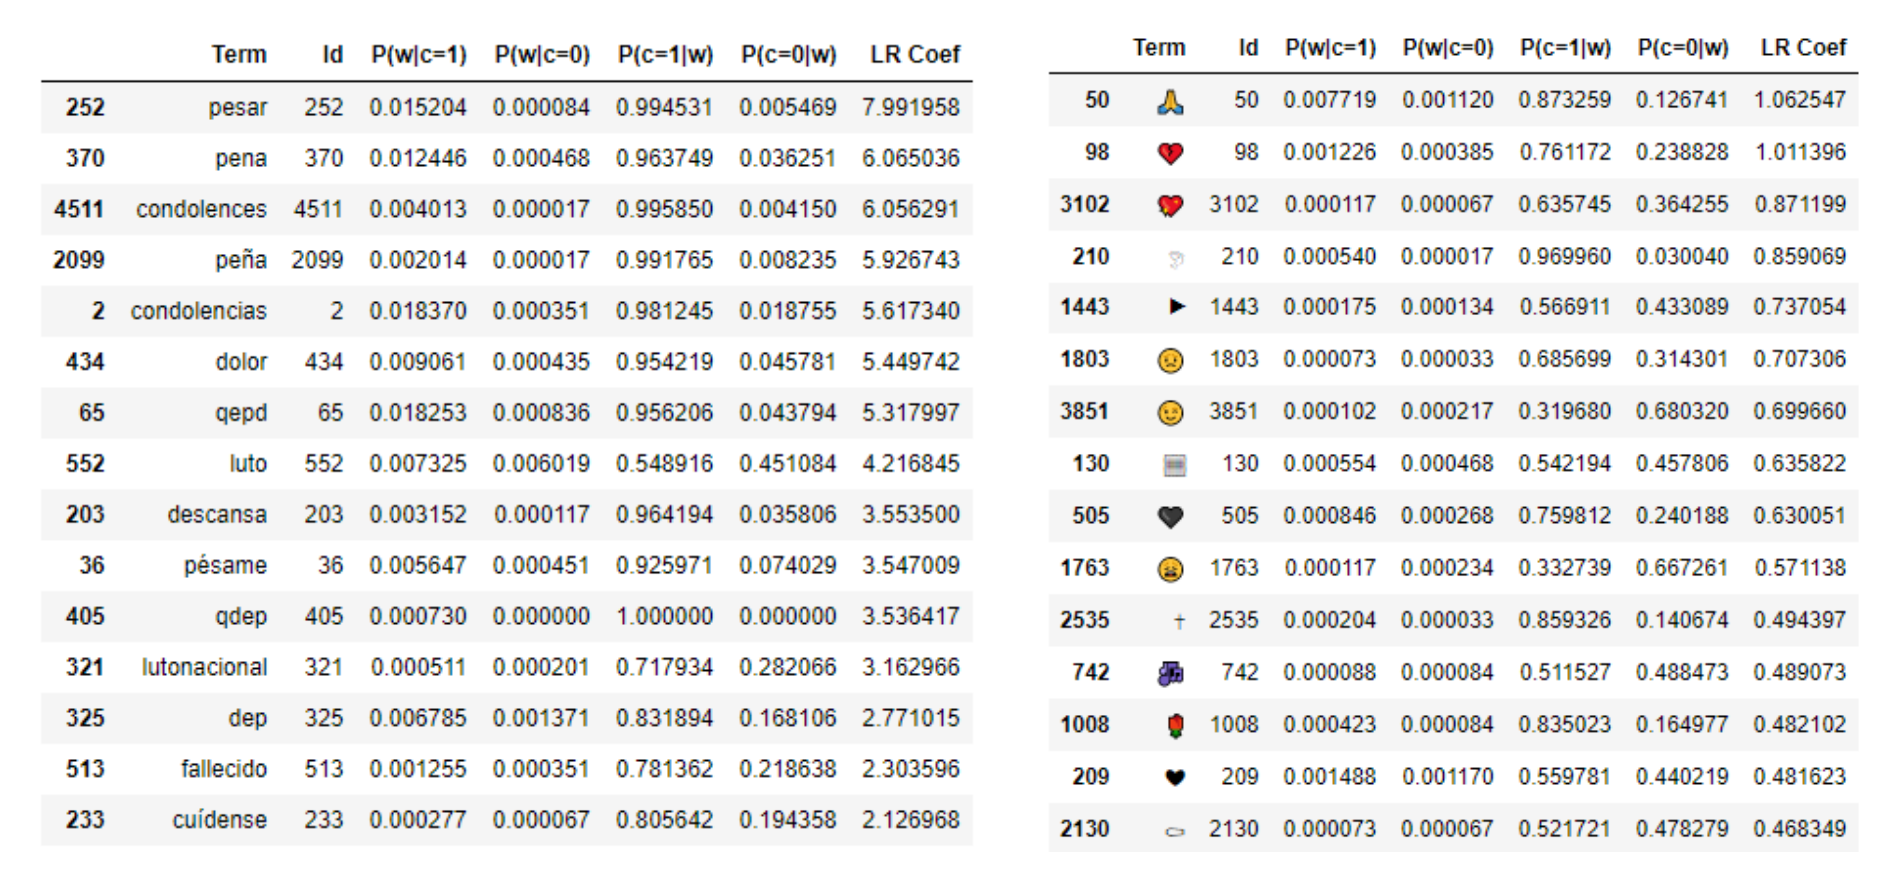
\includegraphics[width=\textwidth]{doc/images/LR_Coef_es.png}
\end{table}

\begin{table}[H]
    \centering
    \caption{Términos con mayor peso dentro de los parámetros de Regresión Logística (LR) en el \textit{dataset} en inglés (EN)}
    \label{tab:lr_coef_en}
    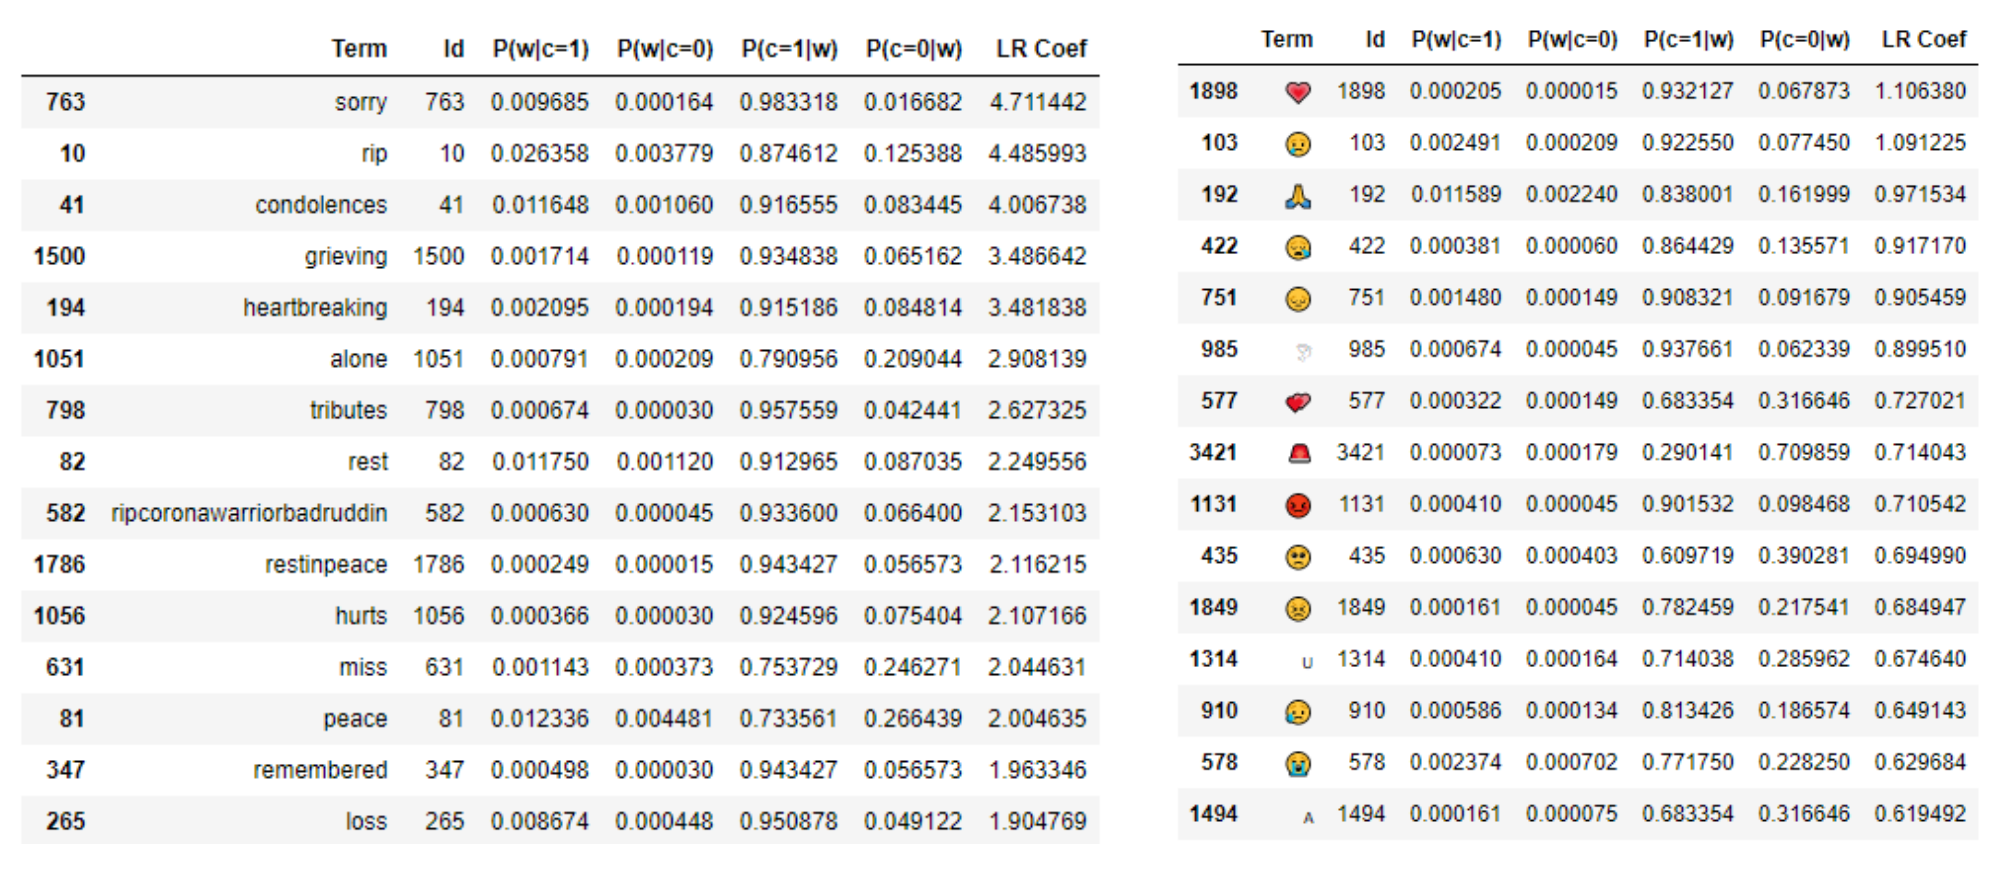
\includegraphics[width=\textwidth]{doc/images/LR_Coef_en.png}
\end{table}

\subsubsection{Random Forest (RF)}

\begin{table}[H]
    \centering
    \caption{Términos con mayor peso dentro de los parámetros de Random Forest (RF) en el \textit{dataset} en español (ES)}
    \label{tab:lr_coef_es}
    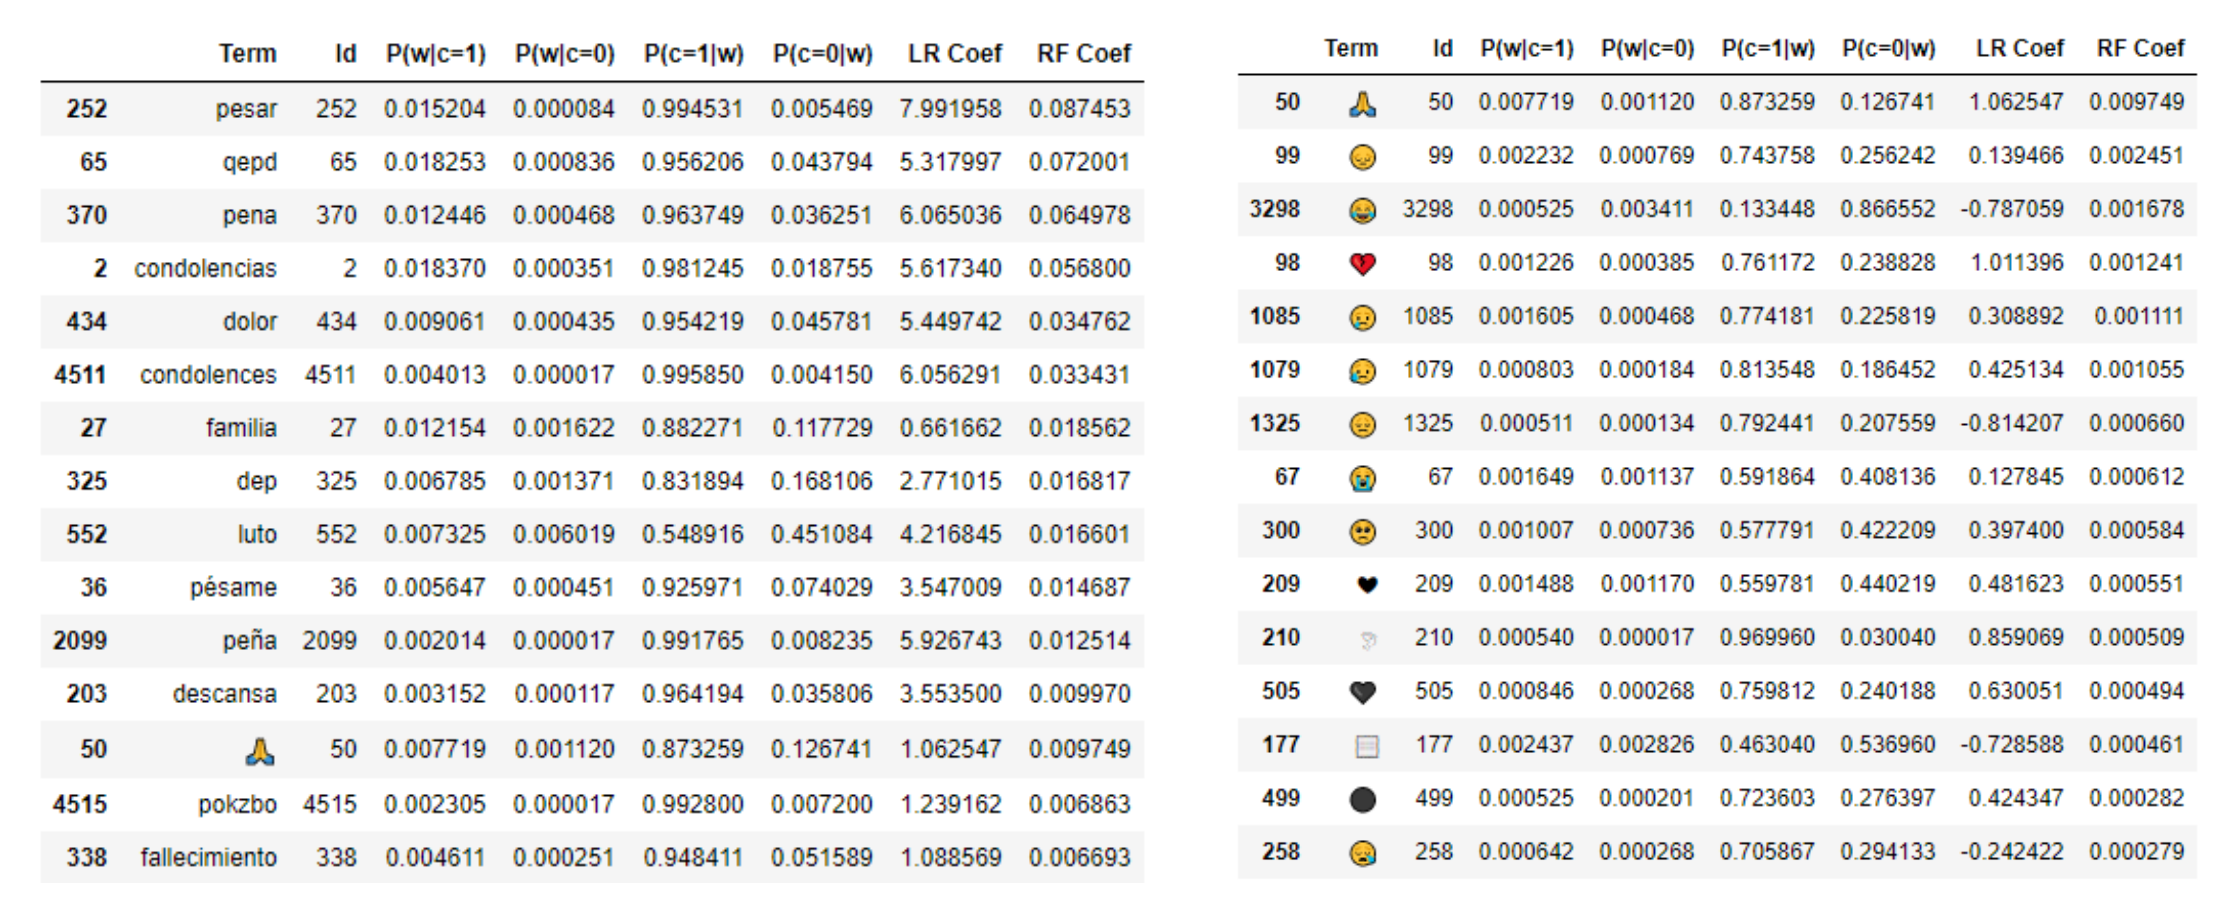
\includegraphics[width=\textwidth]{doc/images/RF_Coef_es.png}
\end{table}

\begin{table}[H]
    \centering
    \caption{Términos con mayor peso dentro de los parámetros de Random Forest (RF) en el \textit{dataset} en inglés (EN)}
    \label{tab:lr_coef_en}
    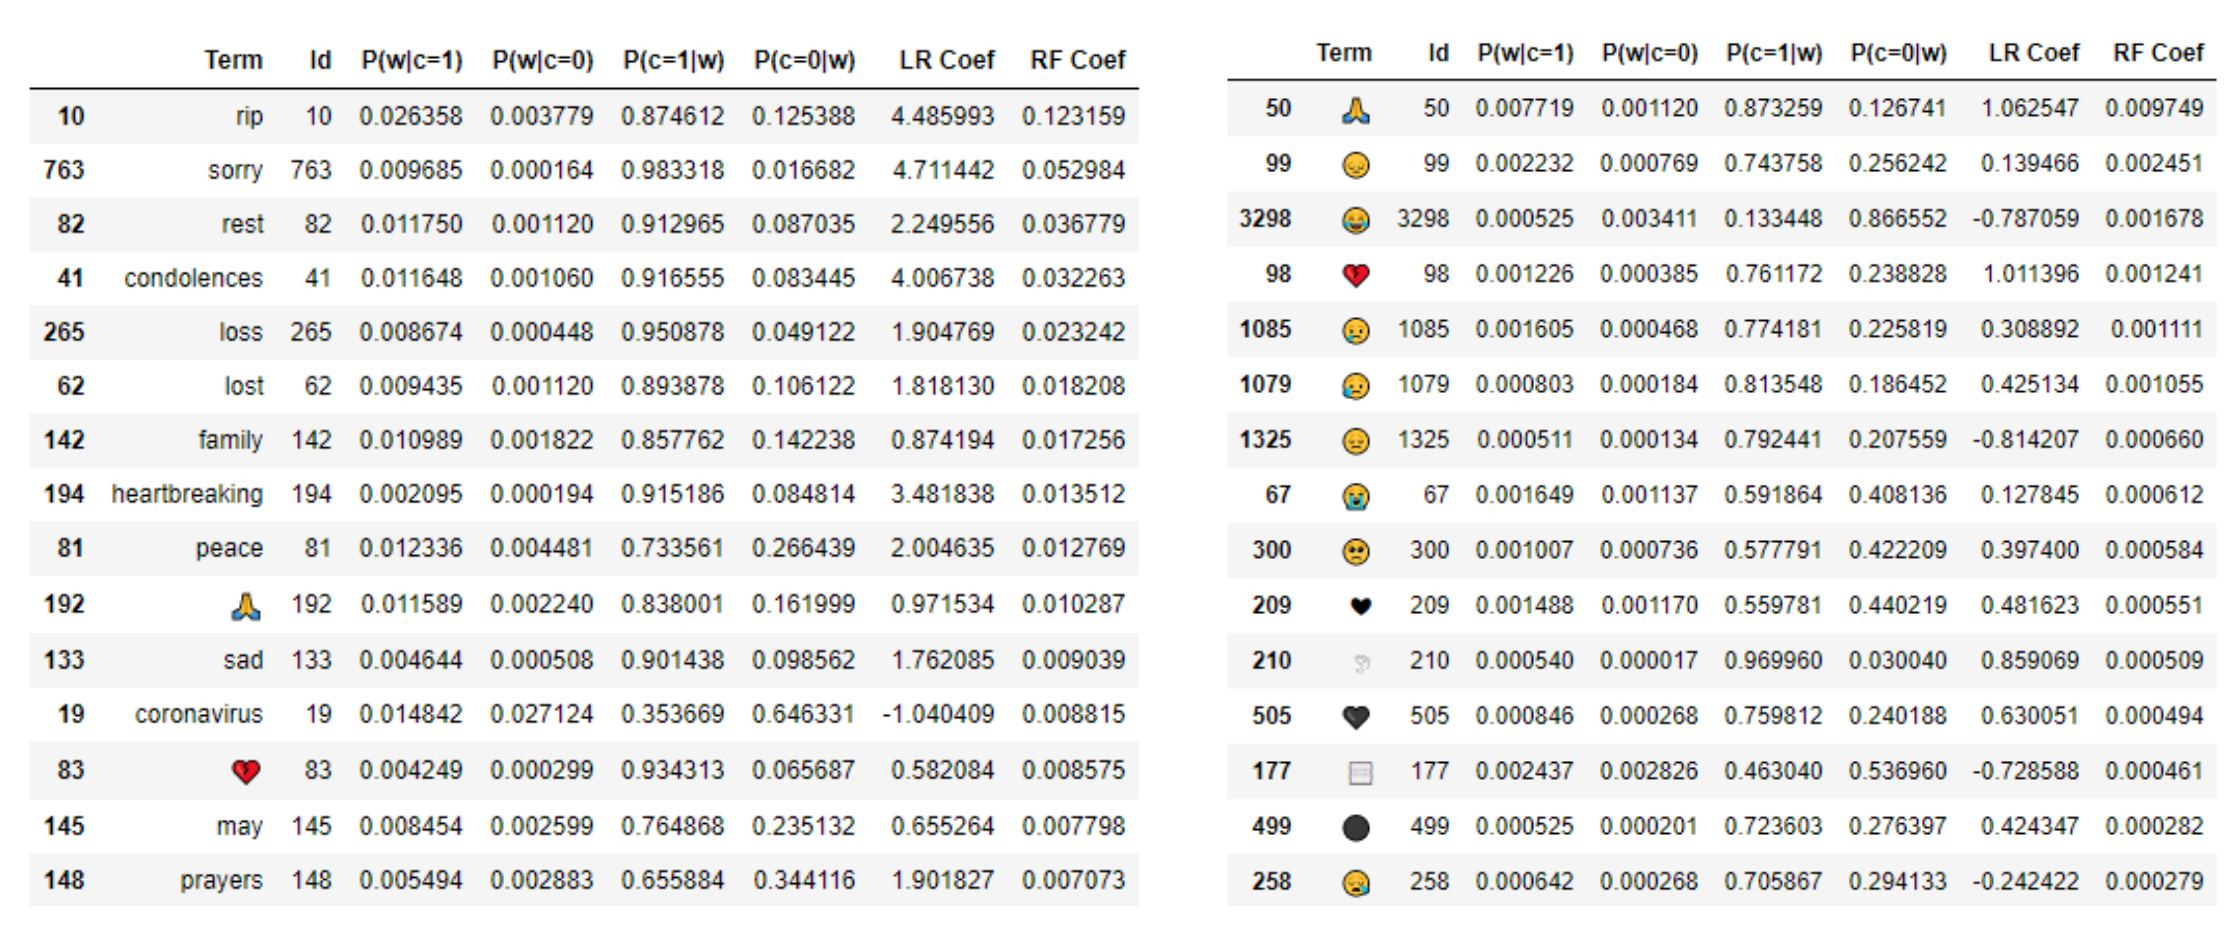
\includegraphics[width=\textwidth]{doc/images/RF_Coef_en.png}
\end{table}